
\chapter{Wireless instrumentation}

One of the most significant technological innovations in industrial instrumentation of late has been the introduction of \textit{radio-based} or \textit{wireless} field instrumentation.  Although this technology is simply too immature at the time of this writing (2011) to displace many wired analog and digital systems, the day is undoubtedly coming when wireless instruments will be one of the major technologies of choice for industrial applications.

Wireless field instruments are naturally digital devices, and as such possess all the innate advantages of digital instrumentation: self-diagnostics, multivariable reporting, duplex communication, etc.  Furthermore, wireless instruments (at least in theory) lack some of the major limitations of wired digital instruments: slow data rates, low node counts, and energy limitations for classified areas.  The single most significant weakness of current wireless field instrument technology appears to be power.  With chemical batteries being the only power source, data update times must be limited to a snail's pace in order to conserve battery life.  With the ongoing development of ``energy harvesting'' devices to locally power wireless field instruments, we may very well see this technology leap ahead of fieldbus and wired-HART instruments.

\vskip 10pt

This chapter focuses on two strands of wireless technology: wireless field instruments (e.g. transmitters, control valves), and long-range wireless data links such as those used in SCADA systems.  At the present time, \textsl{Wireless}HART (IEC standard 62591) is the dominant standard for radio-based field instruments, with multiple manufacturers already offering interoperable products.  Exciting times, these are!  \index{IEC standard 62591 (WirelessHART field instrument communications protocol)}




\filbreak
\section{Radio systems}

``Radio'' systems use electromagnetic fields to communicate information over long distances through open space.  This section explores some of the basic components common to all radio systems, as well as the mathematical analyses necessary to predict the performance of radio communication.



\filbreak
\subsection{Antennas}

A \textit{radio wave} is a form of electromagnetic radiation, comprised of oscillating electric and magnetic fields.  An \textit{antenna}\footnote{For a more detailed discussion of antennas and their electrical characteristics, refer to section \ref{antenna} beginning on page \pageref{antenna}.} is nothing more than a conductive structure designed to emit radio waves when energized by a high-frequency electrical power source, and/or generate high-frequency electrical signals when intercepting radio waves.  Three common antenna designs appear here:

$$\includegraphics{antenna_15.eps}$$

The Yagi antenna, with its ``director'' and ``reflector'' elements fore and aft of the dipole element, exhibits a high degree of \textit{directionality}, whereas the dipole and ``whip'' antennas tend to emit and receive electromagnetic waves equally well in all directions perpendicular to their axes.  Directional antennas are ideal for applications such as radar, and also in point-to-point communication applications.  Omnidirectional antennas such as the dipole and whip are better suited for applications requiring equal sensitivity in multiple directions.  \index{Yagi antenna}  \index{Antenna, Yagi}  \index{Antenna, half-wave}  \index{Dipole antenna, half-wave}  \index{Half-wave dipole antenna}  \index{Antenna, quarter-wave}  \index{Antenna, whip}  \index{Quarter-wave antenna}  \index{Whip antenna}

A photograph of an actual Yagi antenna used in a SCADA system appears here:

$$\includegraphics[width=4in]{antenna_21.eps}$$

\filbreak

The wavelength ($\lambda$) of any wave is its propagation velocity divided by its frequency.  For radio waves, the propagation velocity is the speed of light ($2.99792 \times 10^8$ meters per second, commonly represented as $c$), and the frequency is expressed in Hertz:

$$\lambda = {c \over f}$$

Antenna dimensions are related to signal wavelength because antennas work most effectively in a condition of electrical \textit{resonance}.  In other words, the physical size of the antenna is such that it will electrically resonate at certain frequencies: a \textit{fundamental} frequency as well as the \textit{harmonics} (integer-multiples) of that fundamental frequency.  For this reason, antenna size is inversely proportional to signal frequency: low-frequency antennas must be large, while high-frequency antennas may be small.  \index{Harmonic frequency}  \index{Fundamental frequency}

For example, a quarter-wave ``whip'' antenna designed for a 900 MHz industrial transceiver application will be approximately\footnote{Due to the ``end effect'' of lumped capacitance at the tip of the antenna, an actual quarter-wave antenna needs to be slightly shorter than an actual quarter of the wavelength.  This holds true for dipoles and other antenna designs as well.} 8.3 centimeters in length.  The same antenna design applied to an AM broadcast radio transmitter operating at 550 kHz would be approximately \textit{136 meters} in length!

The following photograph shows a \textit{half-}wave ``whip'' antenna, located at the roofline of a building.  The additional length of this design makes it more efficient than its quarter-wave cousin.  This particular antenna stands approximately one meter in length from connector to tip, yielding a full wavelength value ($\lambda$) of 2 meters, equivalent to 150 MHz:

$$\includegraphics[width=2in]{antenna_22.eps}$$





\filbreak
\subsection{Decibels}

One of the mathematical tools popularly used in radio-frequency (RF) work is the \textit{common logarithm}, used to express power ratios in a unit called the \textit{decibel}.  The basic idea of decibels is to express a comparison of two electrical powers in logarithmic terms.  Every time you see the unit of ``decibel'' you can think: \textit{this is an expression of how much greater (or how much smaller) one power is to another}.  The only question is which two powers are being compared.  \index{Decibel}  \index{Logarithm, common}  \index{Common logarithm}  \index{dB}

Electronic amplifiers are a type of electrical system where comparisons of power are useful.  Students of electronics learn to compare the output power of an amplifier against the input power as a unitless ratio, called a \textit{gain}.  Take for example an electronic amplifier with a signal input of 40 milliwatts and a signal output of 18.4 watts:  \index{Gain, amplifier}

$$\includegraphics{antenna_28.eps}$$

An alternative way to express the gain of this amplifier is to do so using the unit of the \textit{Bel}, defined as the common logarithm of the gain ratio:  \index{Bel}

$$\log \left( P_{out} \over P_{in} \right) = \log \left( 18.4 \hbox{ W} \over 40 \hbox{ mW} \right) = 2.66276 \hbox{ B}$$

When you see an amplifier gain expressed in the unit of ``Bel'', it's really just a way of saying ``The output signal coming from this amplifier is $x$ powers of ten greater than the input signal.''  An amplifier exhibiting a gain of 1 Bel outputs 10 times as much power as the input signal.  An amplifier with a gain of 2 Bels boosts the input signal by a factor of 100.  The amplifier shown above, with a gain of 2.66276 Bels, boosts the input signal 460-fold.

At some point in technological history it was decided that the ``Bel'' (B) was too large and unwieldy of a unit, and so it became common to express powers in fractions of a Bel instead: the \textit{deci}Bel (1 dB = $1 \over 10$ of a Bel).  Therefore, this is the form of formula you will commonly see for expressing RF powers:

$$\hbox{dB} = 10 \log \left( P_{out} \over P_{in} \right)$$

The gain of our hypothetical electronic amplifier, therefore, would be more commonly expressed as 26.6276 dB rather than 2.66276 B, although either expression is technically valid\footnote{It is interesting to note that although the ``Bel'' is a metric unit, it is seldom if ever used without the metric prefix ``deci'' ($1 \over 10$).  One could express powers in microbels, megabels, or any other metric prefix desired, but it is never done in industry: only the decibel is used.}.

\vskip 10pt

\filbreak

An operation students often struggle with is converting a decibel figure back into a ratio, since the concept of logarithms seems to be universally perplexing.  Here I will demonstrate how to algebraically manipulate the decibel formula to solve for the power ratio given a dB figure.

\vskip 10pt

First, we will begin with the decibel formula as given, solving for a value in decibels given a power ratio:

$$\hbox{dB} = 10 \log (\hbox{Ratio})$$

If we wish to solve for the ratio, we must ``undo'' all the mathematical operations surrounding that variable.  One way to determine how to do this is to reverse the order of operations we would follow if we knew the ratio and were solving for the dB value.  After calculating the ratio, we would then take the logarithm of that value, and then multiply that logarithm by 10: start with the ratio, then take the logarithm, then multiply last.  To un-do these operations and solve for the ratio, we must un-do each of these operations in reverse order.  First, we must un-do the multiplication (by dividing by 10):

$${\hbox{dB} \over 10} = {10 \log (\hbox{Ratio}) \over 10}$$

$${\hbox{dB} \over 10} = \log (\hbox{Ratio})$$

Next, we must un-do the logarithm function by applying its mathematical inverse to both sides of the formula -- making each expression a power of 10:

$$10^{\hbox{dB} \over 10} = 10^{\log (\hbox{Ratio})}$$

$$10^{\hbox{dB} \over 10} = \hbox{Ratio}$$

To test our algebra, we can take the previous decibel value for our hypothetical RF amplifier and see if this new formula yields the original gain ratio:

$$\hbox{Ratio} = 10^{\hbox{26.6276 dB} \over 10}$$

$$\hbox{Ratio} = 10^{\hbox{2.66276 B}}$$

$$\hbox{Ratio} = 460$$

Sure enough, we arrive at the correct gain ratio of 460, starting with the decibel gain figure of 26.6276 dB.

\vskip 10pt

\filbreak

We may also use decibels to express power \textit{losses} in addition to power \textit{gains}.  Here, we see an example of a radio-frequency (RF) signal cable losing power along its length\footnote{The dominant mode of energy dissipation in an RF cable is \textit{dielectric heating}, where the AC electric field between the cable conductors excites the molecules of the conductor insulation.  This energy loss manifests as heat, which explains why there is less RF energy present at the load end of the cable than is input at the source end of the cable.}, such that the power out is less than the power in:

$$\includegraphics{antenna_29.eps}$$

$$10 \log \left( P_{out} \over P_{in} \right) = 10 \log \left( 37 \hbox{ mW} \over 40 \hbox{ mW} \right) = -0.3386 \hbox{ dB}$$

Contrasting this result against the previous result (with the amplifier) we see a very important property of decibel figures: any power \textit{gain} is expressed as a \textit{positive} decibel value, while any power \textit{loss} is expressed as a \textit{negative} decibel value.  Any component outputting the exact same power as it takes in will exhibit a ``gain'' value of 0 dB (equivalent to a gain \textit{ratio} of 1).  

Remember that Bels and decibels are nothing more than logarithmic expressions of ``greater than'' and ``less than''.  Positive values represent powers that are \textit{greater} while negative values represent powers that are \textit{lesser}.  Zero Bel or decibel values represent \textit{no change} (neither gain nor loss) in power.

\vskip 10pt

A couple of simple decibel values are useful to remember for approximations, where you need to quickly estimate decibel values from power ratios (or vice-versa).  Each addition or subtraction of 10 dB exactly represents a 10-fold multiplication or division of power ratio: e.g. +20 dB represents a power ratio gain of 10 $\times$ 10 = 100, whereas $-30$ dB represents a power ratio reduction of $1 \over 10$ $\times$ $1 \over 10$ $\times$ $1 \over 10$ = $1 \over 1000$.  Each addition or subtraction of 3 dB approximately represents a 2-fold multiplication or division or power ratio: e.g. +6 dB is approximately equal to a power ratio gain of 2 $\times$ 2 = 4, whereas $-12$ dB is approximately equal to a power ratio reduction of $1 \over 2$ $\times$ $1 \over 2$ $\times$ $1 \over 2$ $\times$ $1 \over 2$ = $1 \over 16$.  We may combine $\pm$ 10 dB and $\pm$ 3 dB increments to come up with ratios that are products of 10 and 2: e.g. +26 dB is approximately equal to a power ratio gain of 10 $\times$ 10 $\times$ 2 $\times$ 2 = 400.

\vskip 10pt

\filbreak

Observe what happens if we combine a ``gain'' component with a ``loss'' component and calculate the overall power out versus power in:

$$\includegraphics{antenna_30.eps}$$

The overall gain of this RF amplifier and cable system expressed as a ratio is equal to the \textit{product} of the individual component gain/loss ratios.  That is, the gain ratio of the amplifier \textit{multiplied} by the loss ratio of the cable yields the overall power ratio for the system:

$$\hbox{Overall gain} = {17.02 \hbox{ W} \over 40 \hbox{ mW}} = (460)(0.925) = 425.5$$

The overall gain may be alternatively expressed as a decibel figure, in which case it is equal to the \textit{sum} of the individual component decibel values.  That is, the decibel gain of the amplifier \textit{added} to the decibel loss of the cable yields the overall decibel figure for the system:

$$\hbox{Overall gain} = 10 \log \left({17.02 \hbox{ W} \over 40 \hbox{ mW}}\right) = 26.6276 \hbox{ dB} + (-0.3386 \hbox{ dB}) = 26.2890 \hbox{ dB}$$

\vskip 10pt

It is often useful to be able to estimate decibel values from power ratios and vice-versa.  If we take the gain ratio of this amplifier and cable system (425.5) and round it down to 400, we may easily express this gain ratio as an expanded product of 10 and 2:

$$425.5 \approx 400 = (10) \times (10) \times (2) \times (2)$$

Knowing that every 10-fold multiplication of power ratio is an addition of +10 dB, and that every 2-fold multiplication of power is an addition of +3 dB, we may express the expanded product as a sum of decibel values:

$$(10) \times (10) \times (2) \times (2) = (10 \hbox{ dB}) + (10 \hbox{ dB}) + (3 \hbox{ dB}) + (3 \hbox{ dB}) = 26 \hbox{ dB}$$

Therefore, our power ratio of 425.5 is approximately equal to +26 decibels.


\vskip 10pt

\filbreak

Decibels always represent comparisons of power, but that comparison need not always be $P_{out} / P_{in}$ for a system component.  We may also use decibels to express an amount of power compared to some standard reference.  If, for example, we wished to express the input power to our hypothetical RF amplifier (40 milliwatts) using decibels, we could do so by comparing 40 mW against a standard ``reference'' power of exactly 1 milliwatt.  The resulting decibel figure would be written as ``dBm'' in honor of the 1 \textit{m}illiwatt reference:  \index{dBm}

$$P_{in} = 10 \log \left( 40 \hbox{ mW} \over 1 \hbox{ mW} \right) = 16.0206 \hbox{ dBm}$$

The unit of ``dBm'' literally means the amount of dB ``greater than'' 1 milliwatt.  In this case, our input signal of 40 milliwatts is 16.0206 dB greater than a standard reference power of exactly 1 milliwatt.  The output power of that amplifier (18.4 watts) may be expressed in dBm as well:

$$P_{out} = 10 \log \left( 18.4 \hbox{ W} \over 1 \hbox{ mW} \right) = 42.6482 \hbox{ dBm}$$

A signal power of 18.4 watts is 42.6482 dB greater than a standard reference power of exactly 1 milliwatt, and so it has a decibel value of 42.6482 dBm.

$$\includegraphics{antenna_31.eps}$$

Notice how the output and input powers expressed in dBm relate to the power gain of the amplifier.  Taking the input power and simply \textit{adding} the amplifier's gain factor yields the amplifier's output power in dBm:

$$P_{in}\hbox{(dB)} + P_{gain}\hbox{(dB)} = P_{out}\hbox{(dB)}$$

$$16.0206 \hbox{ dBm} + 26.6276 \hbox{ dB} = 42.6482 \hbox{ dBm}$$

An electronic signal that begins 16.0206 dB greater than 1 milliwatt, when boosted by an amplifier gain of 26.6276 dB, will become 42.6482 dB greater than the original reference power of 1 milliwatt.

\filbreak

We may alternatively express all powers in this hypothetical amplifier in reference to a 1-watt standard power, with the resulting power expressed in units of ``dBW'' (decibels greater than 1 watt):  \index{dBW}

$$P_{in} = 10 \log \left( 40 \hbox{ mW} \over 1 \hbox{ W} \right) = -13.9794 \hbox{ dBW}$$

$$P_{out} = 10 \log \left( 18.4 \hbox{ W} \over 1 \hbox{ W} \right) = 12.6482 \hbox{ dBW}$$

$$\includegraphics{antenna_32.eps}$$

Note how the input power of 40 milliwatts equates to a negative dBW figure because 40 milliwatts is \textit{less} than the 1 watt reference, and how the output power of 18.4 watts equates to a positive dBW figure because 18.4 watts is \textit{more} than the 1 watt reference.  A positive dB figure means ``more than'' while a negative dB figure means ``less than.''

Note also how the output and input powers expressed in dBW still relate to the power gain of the amplifier by simple addition, just as they did when previously expressed in units of dBm.  Taking the input power in units of dBW and simply \textit{adding} the amplifier's gain factor yields the amplifier's output power in dBW:

$$P_{in}\hbox{(dB)} + P_{gain}\hbox{(dB)} = P_{out}\hbox{(dB)}$$

$$-13.9794 \hbox{ dBW} + 26.6276 \hbox{ dB} = 12.6482 \hbox{ dBW}$$

An electronic signal that begins 13.9794 dB less than 1 watt, when boosted by an amplifier gain of 26.6276 dB, will become 12.6482 dB greater than the original reference power of 1 watt.

\vskip 10pt

\filbreak

This is one of the major benefits of using decibels to express powers: we may very easily calculate power gains and losses by summing a string of dB figures, each dB figure representing the power gain or power loss of a different system component.  Normally, any conflation of \textit{ratios} involves multiplication and/or division of those ratios, but with decibels we may simply add and subtract.  One of the interesting mathematical properties of logarithms is that they ``transform\footnote{In fact, logarithms are one of the simplest examples of a \textit{transform function}, converting one type of mathematical problem into another type.  Other examples of mathematical transform functions used in engineering include the \textit{Fourier transform} (converting a time-domain function into a frequency-domain function) and the \textit{Laplace transform} (converting a differential equation into an algebraic equation).}'' one type of problem into a simpler type: in this case, a problem of multiplying ratios into a (simpler) problem of adding decibel figures.  \index{Transform function}  \index{Fourier transform}  \index{Laplace transform}

\vskip 10pt

For example, we may express the power lost in an RF transmission line (two-conductor cable) in terms of decibels per foot.  Most of this power loss is due to dielectric heating, as the high-frequency electric field of the RF signal causes polarized molecules in the cable insulation to vibrate and dissipate energy in the form of heat\footnote{This is precisely how a microwave oven works: water molecules are polar (that is to say, the electrical charges of the hydrogen and oxygen atoms are not symmetrical, and therefore each water molecule has one side that is more positive and an opposite side that is more negative), and therefore vibrate when subjected to electromagnetic fields.  In a microwave oven, RF energy in the gigahertz frequency range is aimed at pieces of food, causing the water molecules within the food to heat up, thus indirectly heating the rest of the food.  This is a practical example of an RF system where losses are not only expected, but are actually a design objective!  The food represents a load to the RF energy, the goal being complete dissipation of all incident RF energy with no leakage outside the oven.  In RF cable design, however, dissipative power losses are something to be avoided, the goal being complete delivery of RF power to the far end of the cable.}.  The longer the cable, of course, the more power will be lost this way, all other factors being equal.  A type of cable having a loss figure of $-0.15$ decibels per foot at a signal frequency of 2.4 GHz will suffer $-15$ dB over 100 feet, and $-150$ dB over 1000 feet.  To illustrate how decibels may be used to calculate power at the end of an RF system, accounting for various gains and losses along the way using decibel figures: \index{Dielectric heating, RF cable}

$$\includegraphics{antenna_27.eps}$$






\filbreak
\subsection{Antenna radiation patterns}

Different antenna designs are unequal with regard to how well they radiate (and receive) electromagnetic energy.  Every antenna design has a \textit{pattern} of radiation and sensitivity: some directions in which it is maximally effective and other directions where it is minimally effective.  

Some common antenna types and radiation patterns are shown in the following illustrations, the relative radii of the shaded areas representing the degree\footnote{One should not think that the outer edges of the shaded radiation patterns represents some ``hard'' boundary beyond which no radiation is emitted (or detected).  In reality, the radiation patterns extend out to infinity (assuming otherwise empty space surrounding the antenna).  Instead, the size of each shaded area simply represents how effective the antenna is in that direction compared to other directions.  In the case of the vertical whip and dipole antennas, for instance, the radiation patterns show us that these antennas have \textit{zero} effectiveness along the vertical ($Y$) axis centerline.  To express this in anthropomorphic terms, these antenna designs are ``deaf and mute'' in those directions where the radiation pattern is sketched having zero radius from the antenna center.} of effectiveness in those directions away from or toward the antenna:

$$\includegraphics{antenna_23.eps}$$

\filbreak

$$\includegraphics{antenna_24.eps}$$

It should be noted that the radiation patterns shown here are approximate, and may modify their shapes if the antenna is operated harmonically rather than at its fundamental frequency.

\vskip 10pt

A basic principle in antenna theory called \textit{reciprocity} states that the efficiency of an antenna as a radiator of electromagnetic waves mirrors its efficiency as a collector of electromagnetic waves.  In other words, a good transmitting antenna will be a good receiving antenna, and an antenna having a preferred direction of radiation will likewise be maximally sensitive to electromagnetic waves approaching from that same direction.  To use a Yagi as an example:

$$\includegraphics{antenna_16.eps}$$

Related to reciprocity is the concept of equivalent orientation between transmitting and receiving antennas for maximum effectiveness.  The electromagnetic waves emitted by a transmitting antenna are \textit{polarized} in a particular orientation, with the electric and magnetic fields perpendicular to each other.  The same design of antenna will be maximally receptive to those waves if its elements are similarly oriented.  A simple rule to follow is that antenna pairs should always be \textit{parallel} to each other in order to maximize reception, in order that the electric and magnetic fields emanating from the wires of the transmitting antenna will ``link'' properly with the wires of the receiving antenna(s).  If the goal is optimum communication in any direction (omnidirectionality), dipole and whip antennas should be arranged \textit{vertically} so that all antenna conductors will be parallel to each other regardless of their geographic location. 

\filbreak

Yagi antenna pairs may be horizontally or vertically oriented, so long as the transmitting and receiving Yagis are both mounted with the same polarization and face each other.  In industrial SCADA radio applications, Yagi antennas are generally oriented with the dipole wires vertical, so that they may be used in conjunction with omnidirectional whip or dipole antennas.  An illustration of such use is shown here, with multiple ``Remote Terminal Unit'' (RTU) transceivers communicating with a central ``Master Terminal Unit'' (MTU) transceiver:

$$\includegraphics{antenna_17.eps}$$

Here, all the Yagi antennas on the RTUs are vertically oriented, so that they will match the polarization of the MTU's whip antenna.  The Yagi antennas all face in the direction of the MTU for optimum sensitivity.  The MTU -- which must broadcast to and receive from all the RTUs -- really needs an omnidirectional antenna.  The RTUs -- which need only communicate with the one MTU and not with each other -- work best with highly directional antennas.

If the MTU were equipped with a Yagi antenna instead of a whip, it would only communicate well with one of the RTUs, and perhaps not at all with some of the others.  If all RTUs were equipped with whip antennas instead of Yagis, they would not be as receptive to the MTU's broadcasts (lower gain), and each RTU would require greater transmitter power to transmit effectively to the MTU.  

\vskip 10pt

Another important principle to employ when locating any antenna is to keep it far away from any conductive surfaces or objects, including soil.  Proximity to any conductive mass distorts an antenna's radiation pattern, which in turn affects how well it can transmit and receive in certain directions.  If there is any consistent rule to follow when setting up antennas for maximum performance, it is this: \textit{position them as high as possible and as far away from interfering objects as possible!}








\filbreak
\subsection{Antenna gain calculations}

A common way to express the maximal effectiveness of any antenna design is as a ratio compared to some idealized form of antenna with a more uniform radiation pattern.  As with most ratio measurements in radio technology, the standard unit for antenna gain is the \textit{decibel} (dB), related to a ratio of powers as follows:  \index{Decibel}  \index{dB}

$$\hbox{Gain in dB} = 10 \log \left({P \over P_{ref}}\right)$$

The most common reference standard used to calculate antenna gain is a purely theoretical device called an \textit{isotropic antenna}.  This is an ideally omnidirectional antenna having a perfectly spherical radiation pattern:  \index{Isotropic antenna}

$$\includegraphics{antenna_26.eps}$$

If a directional antenna such as a Yagi radiates (and/or receives) 20 times as much power in its most sensitive direction as an isotropic antenna, it is said to have a power gain of 13.01 dBi (13.01 \textit{d}eci\textit{b}els more than an \textit{i}sotropic).  An alternative ``reference'' for comparison is a half-wave dipole antenna.  Decibel comparisons against a dipole are abbreviated dBd.  The assumption of an isotropic antenna as the reference is so common in radio engineering, though, you often see antenna gains expressed simply in units of dB.  The assumption of isotropic reference (dBi) for antenna gain expressions is analogous to the assumption of ``RMS'' measurements in AC circuits rather than ``peak'' or ``peak-to-peak'': if you see an AC voltage expressed without any qualifier (e.g. ``117 volts AC''), it is generally assumed to be an RMS measurement.

Whip antennas typically exhibit an optimal gain of 6 dBi (6 dB being approximately equal to a 4-fold magnification compared to an isotropic antenna), while Yagis may achieve up to 15 dBi (approximately equal to a 32-fold magnification).  Parabolic ``dish'' antenna designs such as those used in microwave communication systems may achieve gains as high as 30 dBi ($\approx$ 1000-fold magnification).  Since antenna gain is not a real amplification of power -- this being impossible according to the Law of Energy Conservation -- greater antenna gain is achieved only by greater \textit{focus} of the radiation pattern in a particular direction.  \index{Conservation of Energy}

\vskip 10pt

The concept of antenna gain is very easy to mis-comprehend, since it is tempting to think of any type of gain as being a true increase in power.  Antenna gain is really nothing more than a way to express how \textit{concentrated} the RF energy of a radiating\footnote{Or -- applying the principle of reciprocity -- antenna gain is really nothing more than a way to express how sensitive a receiving antenna is compared to a truly omnidirectional antenna.} antenna is in one direction compared to a truly omnidirectional antenna.  An analogy to antenna gain is how a horn-style loudspeaker focuses its audio energy more than a loudspeaker lacking a horn.  The horn-shaped speaker \textit{sounds} louder than the horn-less speaker (in one direction only) because its audio energy is more focused.  The two speakers may be receiving the exact same amount of electrical energy to produce sound, but the more directional of the two speakers will be more efficient transmitting sound in one direction than the other.  Likewise, a horn-shaped microphone will have greater sensitivity in one direction than a comparable ``omni'' microphone designed to receive sound equally well from all directions.  Connected to a recording device, the directional microphone seems to present a ``gain'' by sending a stronger signal to the recorder than the omnidirectional microphone is able to send, in that one direction.

The flip-side of high-gain antennas, loudspeakers, and microphones is how poorly they perform in directions other than their preferred direction.  Any transmitting or receiving structure exhibiting a ``gain'' due to its focused radiation pattern must likewise exhibit a ``loss'' in performance when tested in directions other than its direction of focus.  Referring back to directional radio antennas again, a Yagi with an advertised gain of 15 dBi (in its ``preferred'' direction) will exhibit a strong negative gain in the rearward direction where its ability to radiate and receive is almost non-existent.

\vskip 10pt

If even more signal gain is necessary than what may be achieved by narrower radiation focus, an actual electronic amplifier may be added to an antenna assembly to boost the RF power sent to or received from the antenna.  This is common for satellite antenna arrays, where the RF amplifier is often located right at the focal point of the parabolic dish.  Satellite communication requires very high transmitter and receiver gains, due to inevitable signal weakening over the extremely long distances between a ground-based antenna and a satellite antenna in geosynchronous orbit around the Earth.







\filbreak
\subsection{Effective radiated power}

When determining the effectiveness of a radio system, one must include losses in cables, connectors, lightning arrestors, and other elements in the signal path in addition to the antenna itself.  A commonly accepted way to quantify this effectiveness is to rate a radio system against a standard reference consisting of an ideal dipole antenna connected to a 1 milliwatt transmitter with no losses.  Typically expressed in units of decibels, this is called the \textit{Effective Radiated Power}, or \textit{ERP}.  If the ideal antenna model is isotropic instead of a dipole, then the calculation result is called the \textit{Effective Isotropic Radiated Power}, or \textit{EIRP}.  \index{ERP}  \index{EIRP}  \index{Effective Radiated Power (ERP)}  \index{Effective Isotropic Radiated Power (EIRP)} 

Let us consider the following example, where a 2.4 GHz radio transceiver outputs 250 milliwatts\footnote{Actual signal power is typically expressed as a decibel ratio to a reference power of either 1 milliwatt (dBm) or 1 watt (dBW).  Thus, 250 mW of RF power may be expressed as $10 \log {250 \over 1}$ = 23.98 dBm or as $10 \log {0.25 \over 1}$ = $-6.02$ dBW.  Power expressed in unit of dBm will always be 30 dB greater ($1 \times 10^3$ greater) than power expressed in dBW.} of radio-frequency (RF) power to a Yagi antenna through a type LMR 195 coaxial cable 12 feet in length.  A lightning arrestor with 0.5 dB loss is also part of the cable system.  We will assume an antenna gain of 9 dBi for the Yagi and a loss of 0.19 dB per foot for the LMR 195 cable:  \index{Radio Frequency (RF)}  \index{RF}  \index{dBm}  \index{dBW}

$$\includegraphics{antenna_09.eps}$$

The EIRP for this radio system is 30.2 dB: the sum of all gains and losses expressed in decibels.  This means our Yagi antenna will radiate 30.2 dB (1047 times) more RF power in its most effective direction than an isotropic antenna would radiate in the same direction powered by a 1 milliwatt transmitter.  Note that if our hypothetical radio system also included an RF amplifier between the transceiver and the antenna, its gain would have to be included in the EIRP calculation as well.

\vskip 10pt

A practical application of EIRP is how the Federal Communications Commission (FCC) sets limits on radio transmitters within the United States.  Not only is gross transmitter power limited by law within certain frequency ranges, but also the EIRP of a transmitting station.  This makes sense, since a more directional transmitting antenna (i.e. one having a greater gain value) will make it appear as though the transmitter is more powerful than it would be radiating from a less-directional antenna.  If FCC limits were based strictly on transmitter power output rather than EIRP, it might still be possible for an otherwise power-compliant transmitting station to generate excessive interference through the use of a highly directional antenna.  This is why it is illegal, for example, to connect a large antenna to a low-power transmitting device such as a two-way (``walkie-talkie'') radio unit: the two-way radio unit may be operated license-free only because its EIRP is low enough not to cause interference with other radio systems.  If someone were to connect a more efficient antenna to this same two-way radio, its effective radiated power may increase to unacceptable levels (according to the FCC) even though the raw power output by the transmitter circuitry has not been boosted.






\filbreak
\subsection{RF link budget}

Electromagnetic radiation is used as a medium to convey information, to ``link'' data from one physical location to another.  In order for this to work, the amount of signal loss between transmitter and receiver must be small enough that the signal does not become lost in radio-frequency ``noise'' originating from external sources and from within the radio receiver itself.  We may express radio-frequency (RF) power in terms of its comparison to 1 milliwatt: 0 dBm being 1 milliwatt, 3.01 dBm being 2 milliwatts, 20 dBm being 100 milliwatts, etc.  We may use dBm as an absolute measurement scale for transmitted and received signal strengths, as well as for expressing how much ambient RF noise is present (called the ``noise floor'' for its appearance at the bottom of a spectrum analyzer display).  We may use plain dB to express relative gains and losses along the signal path.  \index{Noise floor}

The basic idea behind an ``RF link budget'' is to add \textit{all} gains and losses in an RF system -- from transmitter to receiver with all intermediate elements accounted for -- to ensure there is a large enough difference between signal and noise to ensure good data communication integrity.  If we account all gains as positive decibel values and all losses as negative decibel values, the signal power at the receiver will be the simple sum of all the gains and losses:

$$P_{rx} = P_{tx} + G_{total} + L_{total}$$

\noindent
Where,

$P_{rx}$ = Signal power delivered to receiver input (dBm)

$P_{tx}$ = Transmitter output signal power (dBm)

$G_{total}$ = Sum of all gains (amplifiers, antenna directionality, etc.), a positive dB value

$L_{total}$ = Sum of all losses (cables, filters, path loss, fade, etc.), a negative dB value

\vskip 10pt

This formula tells us how much signal power will be available at the radio receiver, but usually the purpose of calculating a link budget is to determine how much radio transmitter power will be \textit{necessary} in order to have adequate signal strength at the receiver.  More transmitter power adds expense, not only due to transmitter hardware cost but also to FCC licenses that are required if certain power limitations are exceeded.  Excessive transmitter power may also create interference problems with other radio and electronic systems.  Suffice it to say we wish to limit transmitter power to the minimum practical value.

\filbreak

In order for a radio receiver to reliably detect an incoming signal, that signal must be sufficiently greater than the ambient RF noise.  All masses at temperatures above absolute zero radiate electromagnetic energy, with some of that energy falling within the RF spectrum.  This \textit{noise floor} value may be calculated\footnote{Noise power may be calculated using the formula $P_n = kTB$, where $P_n$ is the noise power in watts, $k$ is Boltzmann's constant ($1.38 \times 10^{-23}$ J/K), $T$ is the absolute temperature in Kelvin, and $B$ is the bandwidth of the noise in Hertz.  Noise power usually expressed in units of dBm rather than watts, because typical noise power values for ambient temperatures on Earth are so incredibly small.} or empirically measured using an RF spectrum analyzer as shown in this simulated illustration:  \index{Noise floor}

$$\includegraphics{antenna_11.eps}$$


\filbreak

On top of the ambient noise, we also have the \textit{noise figure} of the receiver itself ($N_{rx}$): noise created by the internal circuitry of the radio receiver.  Thus, the minimum signal power necessary for the receiver to operate reliably ($P_{rx(min)}$) is equal to the decibel sum of the noise floor and the noise figure, by a margin called the minimum \textit{signal-to-noise} ratio:

$$P_{rx(min)} = N_f + N_{rx} + S$$

\noindent
Where,

$P_{rx(min)}$ = Minimum necessary signal power at the receiver input (dBm)

$N_f$ = Noise floor value (dBm)

$N_{rx}$ = Noise figure of radio receiver (dB)

$S$ = Desired signal-to-noise ratio margin (dB)

\vskip 10pt

Substituting this decibel sum into our original RF link budget formula and solving for the minimum necessary transmitter power output ($P_{tx(min)}$), we get the following result:

$$P_{tx(min)} = N_f + N_{rx} + S - (G_{total} + L_{total})$$

\filbreak

It is common for radio receiver manufacturers to aggregate the noise floor, noise figure, and a reasonable signal-to-noise ratio into a single parameter called \textit{receiver sensitivity}.  The ``sensitivity'' of a radio receiver unit is the minimum amount of signal power (usually expressed in dBm) necessary at the input connector for reliable operation despite the inevitable presence of noise.  If we simply express receiver sensitivity as $P_{rx(min)}$ and substitute this term for the sum of noise floor, noise figure, and signal-to-noise margin ($N_f + N_{rx} + S$) in the last formula, we see that the difference in receiver sensitivity (expressed in absolute decibels) and the sum of any gains and losses in the link (also expressed in decibels) tells us the minimum transmitter power required:  \index{Sensitivity, radio receiver}  \index{Noise floor}

$$P_{tx(min)} = P_{rx(min)} - (G_{total} + L_{total})$$

\noindent
Where,

$P_{tx(min)}$ = Minimum necessary transmitter output signal power, in dBm

$P_{rx(min)}$ = Receiver sensitivity (minimum necessary received signal power), in dBm

$G_{total}$ = Sum of all gains (amplifiers, antenna directionality, etc.), a positive dB value

$L_{total}$ = Sum of all losses (cables, filters, path loss, fade, etc.), a negative dB value

\vskip 10pt

For digital radio receivers, sensitivity is a function of error rate: the fewer errors desired, the more signal power required.  To give a practical example, one modern 900 MHz radio transceiver has a specified sensitivity of $-110$ dBm at a bit error rate (BER) of $10^{-4}$ bits (one error for every $10^4$ bits received) and a sensitivity of $-108$ dBm at a BER of $10^{-6}$ bits.  This relationship between signal power and error rate should make intuitive sense: the more powerful the signal compared to any background noise, the more reliably it will be received; the weaker the signal, the more it will become corrupted by noise and therefore the more errors we would expect to see over time.  \index{BER (bit error rate)}  \index{Bit error rate}

\vskip 10pt

\filbreak

Among the losses encompassed in $L_{total}$ are \textit{path loss} and \textit{fade}.  Path loss is the natural loss of signal strength with increasing distance from the radiation source.  As electromagnetic waves propagate outward through space, they inevitably spread.  The degradation in signal strength with increasing distance follows the \textit{inverse square law}\footnote{The inverse square law applies to any form of radiation that spreads from a point-source.  In any such scenario, the intensity of the radiation received by an object from the point-source diminishes with the square of the distance from that source, simply because the rest of the radiated energy misses that target and goes elsewhere in space.  This is why the path loss formula begins with a $-20$ multiplier rather than $-10$ as is customary for decibel calculations: given the fact that the inverse square law tells us path loss is proportional to the square of distance ($D^2$), there is a ``hidden'' second power in the formula.  Following the logarithmic identity that exponents may be moved to the front of the logarithm function as multipliers, this means what would normally be a $-10$ multiplier turns into $-20$ and we are left with $D$ rather than $D^2$ in the fraction.}, where power decreases with the square of distance.  Thus, doubling the distance from transmitting antenna to receiving antenna attenuates the signal by a factor of four ($1 \over {2^2}$, or $-6.02$ dB).  Tripling the distance from transmitting antenna to receiving antenna attenuates the signal by a factor of nine ($1 \over {3^2}$, or $-9.54$ dB).   \index{Path loss, RF}  \index{Inverse square law of radiation} 

\vskip 10pt

Path loss for free-space conditions is a rather simple function of distance and wavelength:

$$L_p = -20 \log \left(4 \pi D \over \lambda\right)$$

\noindent
Where,

$L_p$ = Path loss, a negative dB value

$D$ = Distance between transmitting and receiving antennas

$\lambda$ = Wavelength of transmitted RF field, in same physical unit as $D$

\vskip 10pt

It should be emphasized that this simple path loss formula only applies to completely clear, empty space where the only mechanism of signal attenuation is the natural spreading of radio waves as they radiate away from the transmitting antenna.  Path loss will be significantly greater if any objects or other obstructions lie between the transmitting and receiving antennas.

\vskip 10pt

This same spreading effect also accounts for ``fade,'' where radio waves taking different paths deconstructively interfere (e.g. waves reflected off lateral objects reaching the receiving antenna out-of-phase with the straight-path waves), resulting in attenuated signal strengths in some places (but not in all).  You may have personally experienced fade while driving a vehicle over long distances and listening to an analog (AM or FM) radio: sometimes a particular radio station's signal will ``fade out'' as you drive and then ``fade in'' again while driving in the same direction, for no obvious reason (e.g. no immediate obstructions to the signal).  This is due to radio waves from the station emanating in all directions, then reflecting off of large objects and/or ionized regions high in the earth's atmosphere.  There will inevitably be locations around that station where the incident wave from the transmitting antenna destructively interferes with those reflected waves, the result being regions of ``dead'' space where the signal is much weaker than one would expect from path loss alone.  \index{Fade, RF} 

Fade is a more difficult factor to predict than path loss, and so generally radio system designers include an adequate margin\footnote{``Margin'' is the professionally accepted term to express extra allowance provided to compensate for unknowns.  A more colorful phrase often used in the field to describe the same thing is \textit{fudge factor}.} to account for the effects of fade.  This \textit{fade margin} is typically 20 dB to 30 dB, although it can be greater in scenarios where there are many signal paths due to reflections.  \index{Fade margin, RF}

\filbreak

To illustrate, we will calculate the RF link budget for a 900 MHz radio transmitter/receiver pair directionally oriented toward each other with Yagi antennas.  All sources of signal gain and loss will be accounted for, including the ``path loss'' of the RF energy as it travels through open air.  The gains and losses of all elements are shown in the following illustration:

$$\includegraphics{antenna_10.eps}$$

The path loss value shown in the illustration is a calculated function of the 900 MHz wavelength ($\lambda = {c \over f}$ = 0.3331 meters) and the distance between antennas (500 feet = 152.4 meters), assuming a completely obstruction-free path between antennas:

$$L_p = -20 \log \left(4 \pi (152.4) \over 0.3331\right) = -75.19 \hbox{ dB}$$

According to the receiver manufacturer's specifications, the receiver in this system has a sensitivity of $-75$ dBm, which means our transmitter must be powerful enough to deliver an RF signal at least as strong as $-75$ dBm at the receiver's input connector in order to reliably communicate data.  Inserting this receiver sensitivity figure into our RF link budget formula:

$$P_{tx(min)} = P_{rx(min)} - (G_{total} + L_{total})$$

$$P_{tx(min)} = -75 \hbox{ dBm} - (G_{total} + L_{total})$$

\filbreak

Now we need to tally all the gains and losses between the transmitter and the receiver.  We will use a value of $-20$ dB for fade margin (i.e. our budget will leave room for up to 20 dB of power loss due to the effects of fade):

% No blank lines allowed between lines of an \halign structure!
% I use comments (%) instead, so that TeX doesn't choke.

$$\vbox{\offinterlineskip
\halign{\strut
\vrule \quad\hfil # \ \hfil & 
\vrule \quad\hfil # \ \hfil \vrule \cr
\noalign{\hrule}
%
% First row
\textbf{Gain or Loss} & \textbf{Decibel value} \cr
%
\noalign{\hrule}
%
% Another row
Transmitter cable loss & $-5.64$ dB \cr
%
\noalign{\hrule}
%
% Another row
Transmitter arrestor loss & $-0.5$ dB \cr
%
\noalign{\hrule}
%
% Another row
Transmitter antenna gain & +12.1 dBi \cr
%
\noalign{\hrule}
%
% Another row
Path loss & $-75.19$ dB \cr
%
\noalign{\hrule}
%
% Another row
Fade margin & $-20$ dB \cr
%
\noalign{\hrule}
%
% Another row
Receiver antenna gain & +12.1 dBi \cr
%
\noalign{\hrule}
%
% Another row
Receiver arrestor loss & $-0.5$ dB \cr
%
\noalign{\hrule}
%
% Another row
Receiver cable loss & $-4.23$ dB \cr
%
\noalign{\hrule}
%
% Another row
$G_{total} + L_{total}$ & \textbf{$-$81.86 dB} \cr
%
\noalign{\hrule}
} % End of \halign 
}$$ % End of \vbox

Inserting the decibel sum of all gains and losses into our RF link budget formula:

$$P_{tx(min)} = -75 \hbox{ dBm} - (-81.86 \hbox{ dB})$$

$$P_{tx(min)} = 6.86 \hbox{ dBm}$$

Converting a dBm value into milliwatts of RF power means we must manipulate the dBm power formula to solve for $P_{mW}$:

$$P_{dBm} = 10 \log \left({P_{mW}} \over {1 \hbox{ mW}}\right)$$

$$P_{mW} = 1 \hbox{ mW} \times 10^{\left(P_{dBm} \over 10\right)}$$

$$P_{tx} = 1 \hbox{ mW} \times 10^{\left(6.86 \over 10\right)} = 4.85 \hbox{ milliwatts}$$

At this point we would do well to take stock of the assumptions intrinsic to this calculation.  Power gains and losses inherent to the components (cables, arrestors, antennas) are quite certain because these are tested components, so we need not worry about these figures too much.  What we know the least about are the environmental factors: noise floor can change, path loss \textit{will} differ from our calculation if there is any obstruction near the signal path or under certain weather conditions (e.g. rain or snow dissipating RF energy), and fade loss is known to change dynamically as moving objects (people, vehicles) pass anywhere between the transmitter or receiver antennas.  Our RF link budget calculation is really only an estimate of the transmitter power needed to get the job done.  \index{Noise floor}

How then do we improve our odds of building a reliable system?  One way is to over-build it by equipping the transmitter with more power than the most pessimistic link budget predicts.  However, this can cause other problems such as interference with nearby electronic systems if we are not careful.  A preferable method is to conduct a \textit{site test} where the real equipment is set up in the field and tested to ensure adequate received signal strength.  






\filbreak
\subsection{Link budget graph}

Many of the concepts previously explored may be represented in a single graph\footnote{I am indebted to Eric McCollum, Kei Hao, Shankar V. Achanta, Jeremy Blair, and David Kechalo for presenting this form of diagram in a technical paper presented at the 45th annual Western Protective Relay Conference in Spokane, Washington in October of 2018.  I do not know if these authors are responsible for the invention of this form of graph, but it was certainly the first time I encountered one like it, and it so clearly showed all the fundamental quantities of an RF link budget that I had to include something similar in my book!}, showing RF signal strength as a function of physical position within the RF link (from transmitter to receiver).  The horizontal axis of this graph represents the position along the link path from transmitter to receiver, while the vertical axis represents RF signal strength in dBm:

$$\includegraphics{antenna_33.eps}$$

At the very bottom of this graph we see the noise floor, representing natural RF noise that is unavoidable.  Above that we see the added noise figure and signal/noise ratios summing up to a higher line representing the receiver's sensitivity, which is the minimum amount of signal power it must receive in order to reliably function.

Near the top of this graph we see a series of thicker line segments representing the various losses and gains within the system.  Single-point losses such as lightning arrestors appear as vertical downward steps, while progressive losses such as cables and path loss appear as downward slopes.  Single-point gains such as antennas appear as vertical upward steps.  Note where EIRP appears on this graph: the amount of signal power at the transmitting antenna's output, factoring in the antenna's gain as well as any losses between the transmitter and the transmitting antenna.  As previously mentioned, the Federal Communications Commission (FCC) sets regulatory limits for EIRP in the United States, because if only the transmitter's output power were regulated, it would be possible to thwart that limit using high-gain antennas.

At the far right-hand end of the graph, we see the difference between the receiver's input signal power and the receiver's sensitivity as a \textit{margin} for the link budget.  This margin must exist in order to grant the system tolerance to unexpected power losses such as those resulting from inclement weather, interference from objects within the link path, cable deterioration, coupling corrosion, increases in noise floor, etc.




\filbreak
\subsection{Fresnel zones}

One of the many factors affecting RF link power transfer from transmitter to receiver is the openness of the signal path between the transmitting and receiving antennas.  As shown in the previous subsection, \textit{path loss} is relatively simple to calculate given the assumption of totally empty space between the two antennas.  With no obstacles in between, path loss is simply a consequence of wave dispersion (spreading).  Unless we are calculating an RF link budget between two airplanes or two spacecraft, though, there really is no such thing as totally empty space between the transmitting and receiving antennas.  Buildings, trees, vehicles, and even the ground are all objects potentially disrupting what would otherwise be completely open space between transmitter and receiver.

A common expression in microwave radio communication is \textit{line-of-sight}, or \textit{LoS}.  The very wording of this phrase evokes an image of being able to see a straight path between transmitting and receiving antennas.  Obviously, if one does not have a clear line-of-sight path between antennas, the signal path loss will definitely be more severe than through open space.  However, a common error is in thinking that the mere existence of an unobstructed straight line between antennas is all that is needed for unhindered communication, when in fact nothing could be further from the truth:  \index{Line of Sight (RF)}

$$\includegraphics{antenna_12.eps}$$

In fact, the free space necessary to convey energy in electromagnetic wave form takes on the form of football-shaped zones: the first one solid followed by annular (hollow) zones concentrically surrounding the first.  These elliptical volumes are called \textit{Fresnel zones}:   \index{Fresnel zone}

$$\includegraphics{antenna_13.eps}$$

The precise shapes of these Fresnel zones are a function of wavelength and distance between antennas, \textit{not} the size or configurations of the antennas themselves.  In other words, you cannot change the Fresnel zone sizes or shapes by merely altering antenna types.  This is because the Fresnel zones do not actually map the distribution of electromagnetic fields, but rather map the free space we need to keep clear between antennas\footnote{The physics of Fresnel zones is highly non-intuitive, rooted in the wave-nature of electromagnetic radiation.  It should be plain to see, though, that Fresnel zones cannot describe the actual electromagnetic field pattern between two antennas, because we know waves tend to spread out over space while Fresnel zones converge at each end.  Likewise, Fresnel zones vary in size according to the distance between two antennas which we know radiation field patterns do not.  It is more accurate to think of Fresnel zones as \textit{keep-clear} areas necessary for reliable communication between two or more antennas rather than actual field patterns.}.

If any object protrudes at all into any Fresnel zone, it diminishes the signal power communicated between the two antennas.  In microwave communication (GHz frequency range), the inner-most Fresnel zone carries most of the power, and is therefore the most important from the perspective of interference.  Keeping the inner-most Fresnel zone absolutely clear of interference is essential for maintaining ideal path-loss characteristics (equivalent to open-space).  A common rule followed by microwave system designers is to try to maintain an inner Fresnel zone that is at least 60\% free of obstruction.

In order to design a system with this goal in mind, we need to have some way of calculating the width of that Fresnel zone.  Fortunately, this is easily done with the following formula:

$$r = \sqrt{{n \lambda d_1 d_2} \over D}$$

\noindent
Where,

$r$ = Radius of Fresnel zone at the point of interest

$n$ = Fresnel zone number (an integer value, with 1 representing the first zone)

$d_1$ = Distance between one antenna and the point of interest

$d_2$ = Distance between the other antenna and the point of interest

$D$ = Distance between both antennas

$\lambda$ = Wavelength of transmitted RF field, in same physical unit as $D$, $d_1$, and $d_2$

\vskip 10pt

Note: the units of measurement in this formula may be any unit of length, so long as they are all the same unit.

$$\includegraphics{antenna_14.eps}$$

\filbreak

To illustrate by example, let us calculate the radius of the first Fresnel zone for two microwave antennas operating at 2.4 GHz, separated by one mile (1.609 km), at the widest portion of that zone.  The wavelength of a 2.4 GHz signal is 0.1249 meters, from the formula $\lambda = {c \over f}$.  Distances $d_1$ and $d_2$ will both be equal to one-half of the total distance, since the widest portion of the Fresnel zone will be exactly at its mid-point between the two antennas ($d_1 = d_2$ = 804.7 meters).  Here, we solve for $r$ as follows:

$$r = \sqrt{{n \lambda d_1 d_2} \over D}$$

$$r = \sqrt{{(1) (0.1249) (804.7^2)} \over 1609}$$

$$r = 7.089 \hbox{ meters}$$

Consider for a moment the significance of this dimension.  At the very least, it means the antennas must be mounted this high off the ground in order to avoid having the most important Fresnel zone contact the earth itself (assuming level terrain), not to mention any objects above ground level such as buildings, vehicles, or trees between the two antennas.  Consider also that the Fresnel zone is football-shaped, and therefore this 7.089 meter radius extends horizontally from the centerline connecting both antennas as well as vertically.  This means that in order for this Fresnel zone to be untouched, there must be a clear path \textit{14.18 meters wide} in addition to the antennas being at least 7.089 meters off the ground!  If we were to consider a 900 MHz signal -- another common frequency for industrial wireless devices -- the minimum height above ground would be 11.58 meters, and the minimum clear path width 23.16 meters!  

\vskip 10pt

As you can see, ``line of sight'' is not as simple as it may first appear.







\filbreak
\section{\textsl{Wireless}HART}

\label{WirelessHART}

An exciting development in industrial instrumentation is the \textsl{Wireless}HART radio communication standard, specifically designed for field instrument use (e.g. transmitters, valve positioners) as opposed to general data communication.  The IEC (International Electrotechnical Commission) has codified the \textsl{Wireless}HART standard as IEC 62591. \index{IEC standard 62591 (WirelessHART field instrument communications protocol)}



\filbreak
\subsection{Introduction to \textsl{Wireless}HART}

\textsl{Wireless}HART is a subset of the HART industrial instrument communication standard as of version 7, communicating process data over 2.4 GHz radio waves.  Individual instruments communicate with a common ``gateway'' device serving as an interface between the wireless network and a wired network or a host control system.  In addition to this, though, individual \textsl{Wireless}HART devices also form links with one another, so that the network data routes look like a ``mesh'' with all nearby nodes interconnected in addition to connecting with the gateway:  \index{WirelessHART}

$$\includegraphics{wirelesshart_01.eps}$$

In a mesh network, devices (nodes) perform double-duty as \textit{repeaters} to relay data from other instruments to the gateway as needed.  In other words, data transmitted from one \textsl{Wireless}HART instrument may not be directly received by the gateway device if that path is blocked or too far away.  Instead, the data may ``hop'' from one device to another nearby, which then re-broadcasts that information to the gateway via a clearer path.

The purpose of a mesh network is to provide redundant data pathways in case of device failure or changes in the environment interrupting radio communication between devices.  In this way, data packets may be re-routed to the gateway if the shortest route fails, in a manner similar to how Terminal Control Protocol (TCP) and Internet Protocol (IP) work together to route data segments from source to destination over the ``mesh'' of the Internet.  This feature is often referred to in \textsl{Wireless}HART technical literature as the \textit{self-healing} property of the mesh network.

According to the HART Foundation, reliability for a well-designed \textsl{Wireless}HART mesh network is 99.7300204\% minimum, and typically greater than 99.9999998\%.

With each \textsl{Wireless}HART field instrument capable of functioning as a radio repeater, the potential exists to form wireless networks larger in size than the maximum broadcast/reception range of any one device.  This illustration shows what is possible\footnote{Some obvious connecting paths between field devices have been omitted from this illustration if the path length exceeds a certain maximum distance.  As you can see, the instruments in the far-left cluster \textit{must} rely on data packet relaying by instruments closer to the gateway, since they themselves are too far away from the gateway to directly communicate.}:  

$$\includegraphics{wirelesshart_02.eps}$$

\vskip 10pt

\filbreak

An important consideration when planning a \textsl{Wireless}HART network is battery life.  With the main purpose of wireless field instruments being the elimination of wired connections to the host system, the field instruments cannot rely on a host system for their electrical power needs.  Lithium-based batteries currently fulfill this role as primary\footnote{Another exciting technological development paralleling the implementation of \textsl{Wireless}HART in industry is that of \textit{energy-harvesting} devices to generate DC electricity from nearby energy sources such as vibrating machines (mechanical motion), hot pipes (thermal differences), photovoltaic (solar) panels, and even small wind generators.  Combined with rechargeable batteries to sustain instrument operation during times those energy sources are not producing, energy-harvesters promise great extension of battery life for wireless instruments of all types.} power source, with life expectancies of several years.  Interestingly, the amount of energy required by a \textsl{Wireless}HART device to transmit radio-frequency data is small compared to the energy required to power its essential instrument functions (e.g. pressure measurement, temperature measurement).  This means a \textsl{Wireless}HART device operating as a radio repeater (in addition to being a measurement device) adds little burden to its battery.

\vskip 10pt

Perhaps the greatest challenge in sustaining any wireless field instrument network is ensuring network integrity despite unending changes in the physical environment around the instruments.  Remember that this is an \textit{industrial}, field-instrument wireless network designed to be installed in less-than-ideal physical environments.  These wireless devices must somehow reliably communicate with each other despite interference from high-power electrical devices (e.g. variable-frequency motor drive units), while mounted on or near metal objects such as girders, pipes, pipe racks, large vessels, motors, enclosures, shelters, and electrical conduits.  Even the ground of an industrial environment can be an impediment to robust radio communication: steel-reinforced concrete and electrical grounding grids form what is essentially a solid ``ground plane'' that will interfere with \textsl{Wireless}HART devices mounted too close to ground level.  Added to all this spatial complexity is the continual presence of large vehicles and other moving machines (cranes, forklifts, manlifts, etc.).  It is not uncommon for scaffolding to be temporarily erected for maintenance work in industrial areas, presenting yet one more obstacle for RF signals.  \index{Variable-frequency drive}  \index{VFD}

In answer to these challenges is an integral and essential component of a \textsl{Wireless}HART network called the \textit{Network Manager}: an advanced digital algorithm usually executed by the network gateway's microprocessor.  The purpose of the Network Manager is to manage the details of the network automatically, ``tuning'' various parameters for optimum reliability and data throughput.  Among other tasks, the Network Manager assigns ``timeslots'' for individual devices to transmit, determines the frequency-hopping schedule, detects and authenticates new devices added to the network, dynamically adjusts device transmission power, and selects alternative routes between devices.  \index{Network Manager, WirelessHART}

In a sense, the Network Manager in a \textsl{Wireless}HART network continually audits and tunes the RF system in an attempt to maximize reliability.  The Network Manager's functionality does not substitute for good planning during the design phase of the \textsl{Wireless}HART network, but it does eliminate the need for a human technician or engineer to continuously monitor the network's performance and make the small adjustments necessary to compensate for changing conditions.  When changes occur in a \textsl{Wireless}HART network that cannot be compensated by the Network Manager, the real-time statistics provided by the Network Manager are invaluable to the technician or engineer assigned to update the network.




\filbreak
\subsection{\textsl{Wireless}HART network protocol}

The OSI reference model will be used here to identify and describe various features of the \textsl{Wireless}HART protocol.


\subsubsection{Physical Layer}

\begin{itemize}
\item 2.4 GHz to 2.5 GHz (``ISM'' -- Industrial, Scientific, Medical) signal band
\item O-QPSK modulation (offset quadrature phase-shift keying)
\item 250 kbps data rate
\item Direct-sequence spread-spectrum (DSSS) with frequency-hopping between 15 channels within that band for security and interference reduction
\item Variable transmit power, with 10 dBm (10 milliwatts) being default
\end{itemize}

\index{Spread-spectrum radio}

\textsl{Wireless}HART uses 2.4 GHz (nominal) as its transmission frequency and low power levels (10 dBm nominal) because meeting these criteria allows \textsl{Wireless}HART devices to be unlicensed according to FCC (Federal Communications Commission) standards.  If \textsl{Wireless}HART fell outside of these limits, the FCC would require end-users to obtain and maintain licenses for the use of these devices and licenses for maintenance personnel installing and maintaining the devices.  Such requirements would make \textsl{Wireless}HART prohibitively expensive for all but the most challenging applications and thereby limit its marketability.  \index{FCC -- Federal Communications Commission}  \index{Federal Communications Commission}  \index{ISM 2.4 GHz radio band}

The purpose of variable transmit power (as scheduled by the Network Manager) is to conserve battery life: an important priority for instruments whose main (or even sole) source of energy is a battery with a finite life.  A secondary benefit of this power-limiting feature is that the interference potential of a \textsl{Wireless}HART network on other wireless devices sharing the same 2.4 GHz band is further minimized.




\filbreak
\subsubsection{Data Link Layer}

\begin{itemize}
\item TDMA (Time-Division Multiple Access) bus arbitration, with 10-millisecond timeslots allocated for device transmission
\item Network ID number uniquely identifies each \textsl{Wireless}HART network, allowing multiple networks to overlap the same physical area
\item Channel ``blacklisting'' -- automatically avoids hopping to noisy channels
\end{itemize}

TDMA bus arbitration means that the Network Manager plans and schedules the transmission times of all field devices, giving each one its own dedicated time to ``speak.''  With these non-overlapping timeslots scheduled and broadcast to all the field devices, collisions are prevented while at the same time ensuring determinism (the guarantee that data packets \textit{will} reach their destination within a certain specified time) barring any physical interruption of the data path.  \index{Determinism, network}




\filbreak
\subsubsection{Network Layer}

\begin{itemize}
\item ``Mesh'' networking -- devices automatically establish links with any other nearby \textsl{Wireless}HART devices
\item Signal repeating -- devices may act as ``repeaters'' for other devices too far away from the master unit
\item A \textit{Network Manager} device determines communication routes between field devices, as well as timing schedules  \index{Network Manager, WirelessHART}
\item Four levels of data message priority (listed from highest to lowest):
\subitem \textbf{Command}: network management messages
\subitem \textbf{Process data}: PV values
\subitem \textbf{Normal}: \textit{all messages other than Command, Process, or Alarm}
\subitem \textbf{Alarm}: messages reporting device alarms and events
\end{itemize}

The Network Manager in a \textsl{Wireless}HART network plays a role similar to the Link Active Scheduler (LAS) in a FOUNDATION Fieldbus network segment.  The Network Manager assigns time-slots for individual devices to communicate, determines alternative communication routes (i.e. it designs and continually updates the mesh), and continually adjusts device transmit power in order to ensure optimal operation.  This dynamic management of the wireless network is critically important in order to maintain low data latency times and high reliability in the face of changing environment variables such as objects coming into and out of the radio pathways (e.g. cranes, trucks, forklifts, man-lifts, scaffolding, and any other large metal structures which may temporarily alter the RF environment in an industrial setting.).  Like FOUNDATION Fieldbus LAS devices, multiple (redundant) Network Managers are possible within a \textsl{Wireless}HART network with only one being active at any time.



\filbreak
\subsubsection{Application Layer}

\begin{itemize}
\item 128-bit encryption of data
\item Backward-compatibility with wired-HART command structure and DDL (Device Description Language)
\end{itemize}

The backward compatibility of \textsl{Wireless}HART with wired-HART field instruments is an incredibly valuable feature of this standard, as it opens the door to wireless integration of legacy HART instruments.  All that is needed to make a wired-HART instrument part of a functioning \textsl{Wireless}HART network is to attach the appropriate adapter, such as Emerson's \textit{THUM}.  Essentially, this step adds an antenna (and associated network interface electronics) on any legacy HART instrument, enabling it to communicate with native \textsl{Wireless}HART instruments and with the wireless gateway.  This backward compatibility also improves integration of \textsl{Wireless}HART instruments, as they may communicate with legacy HART software application just as easily as wired-HART devices can.  This means programs such as Emerson's AMS are able to interrogate \textsl{Wireless}  \index{Emerson THUM WirelessHART adapter}HART instruments just as easily as they can wired-HART instruments, with no changes to the program code.

\vskip 20pt

\filbreak

Other wireless networking protocols exist which are similar but not identical to \textsl{Wireless}HART.  A few are listed here in contrast for better understanding.




\subsubsection{\textsl{Wireless}HART versus Bluetooth}

Bluetooth is a popular wireless communication standard used in personal computing and other personal electronic devices such as cell phone headsets.

Like \textsl{Wireless}HART, Bluetooth supports channel-hopping and uses TDMA arbitration.  However, Bluetooth uses a much simpler \textit{star} network topology: up to seven Bluetooth slave devices may communicate with one Bluetooth master device.  By contrast, \textsl{Wireless}HART allows for a greater number of field devices communicating with one Network Manager device, and the network topology is \textit{mesh}, where any device may transmit data to any other device on the same network and have that other device ``repeat'' the data to the Network Manager.  \index{Spread-spectrum radio}





\filbreak
\subsubsection{\textsl{Wireless}HART versus ZigBee}

ZigBee is a mesh-networking wireless communication standard which has found application in building automation systems.  It applies the IEEE 802.15.4-2006 standard for both Physical and Data Link layers, whereas \textsl{Wireless}HART employs its own unique Data Link layer including features such as channel ``blacklisting'' and time-slot synchronization to avoid collisions.

A major difference between ZigBee and \textsl{Wireless}HART is the methods of channel arbitration used: ZigBee uses CSMA/CA while \textsl{Wireless}HART uses TDMA.  Time Division arbitration tends to be more time-efficient (and certainly more deterministic) when large numbers of devices are within range of each other.





\filbreak
\subsubsection{\textsl{Wireless}HART versus Wi-Fi}

Wi-Fi (IEEE 802.11) is a wireless communication standard that is extremely popular for personal computer Internet access.  Unlike \textsl{Wireless}HART, Wi-Fi does not support channel-hopping for security and interference reduction.  Wi-Fi, like ZigBee, also uses CSMA/CA channel arbitration, while \textsl{Wireless}HART uses TDMA channel arbitration to achieve determinism.






\filbreak
\subsection{\textsl{Wireless}HART network gateway device}

The \textit{Network Gateway} is a critically important component in a \textsl{Wireless}HART system.  It is the sole channel through which all field device data funnels to the host control system.  Physically, a network gateway is nothing more than a box with an antenna on it, and connections within for electrical power and wired networks (e.g. Ethernet, EIA/TIA-485).  Shown here is an Emerson model 1420\footnote{The model 1420 gateway has been superseded by the Smart Wireless Gateway, also manufactured by Emerson.} ``Smart Wireless Gateway'':  \index{Emerson model 1420 WirelessHART gateway}  \index{Emerson Smart Wireless Gateway}  \index{Ethernet}  

$$\includegraphics[width=3in]{wirelesshart_04.eps}$$

Electrically, these devices are quite complex.  They are microprocessor-controlled, and often serve as the physical host for the Network Manager algorithm: orchestrating and tuning the wireless network communications.

\filbreak

Since \textsl{Wireless}HART is a purely \textit{digital} communication standard, all data points from the field devices are stored in the gateway in digital form, and must be accessed digitally.  In the case of Emerson's Smart Wireless Gateway, the data may be accessed by any host system via Modbus query commands, communicated either serially (EIA/TIA-485, Modbus RTU format) or encapsulated in Ethernet packets (Modbus TCP).  Screw terminal connections exist on the Emerson gateway for an EIA/TIA-485 (RS-485) cable to connect, as well as multiple RJ-45 Ethernet ports for connection to a hub or switch where other Ethernet-based computers and systems may connect as well:  \index{Modbus RTU}  \index{Modbus TCP}

$$\includegraphics[width=3in]{wirelesshart_06.eps}$$

Like so many other industrial Ethernet-ready devices, the Emerson Smart Wireless Gateway has a built-in web server, allowing password-protected access to configuration pages using nothing more than a personal computer with Ethernet connectivity and a web (Internet) browser program.  Simply type the IP address of the gateway port into the browser's URL field, and the personal computer will connect to the gateway.

\filbreak

Individual device data points are custom-mapped by the user to specific Modbus registers inside the gateway's memory, as shown on this configuration page:

$$\includegraphics{wirelesshart_07.eps}$$

In this screenshot we see the primary variables\footnote{Device variables are addressed at the network gateway level by the device's HART tag (long tag, not short tag) and internal device variable name.  Thus, the primary variable (\texttt{PV}) of temperature transmitter \texttt{TEMP2} is specified as \texttt{TEMP2.PV} using a period symbol (\texttt{.}) as the delimiting character between the device name and the internal variable name.} (PV) of two Rosemount model 648 \textsl{Wireless}HART temperature transmitters mapped to Modbus registers 30001 and 30002.  It should be noted that all \textsl{Wireless}HART field instruments are multi-variable devices, and as such are capable of reporting more than one variable to the gateway.  If anyone were interested, it would have been possible in this example to assign battery voltage as a secondary variable (SV), tertiary variable (TV), or quaternary variable (QV) inside one or both temperature transmitters, then map those data points to their own Modbus registers in the gateway so that a host system could access and monitor battery voltage for the field instruments.  Just as in wired-HART communication, multi-variable data communication from each transmitter is possible.  This is not often done as a regular course of action with wired-HART instruments due to the very slow data rate of wired HART (1200 bps).  However, with the much faster data rate of \textsl{Wireless}HART (250 kbps), the extra time required for a field instrument to transmit three or four variables instead of just one variable is insignificant with respect to the needs of process measurement and control.

\filbreak

The next screenshot shows a portion of a simple PLC program written to query these two Modbus registers inside the Emerson gateway.  The PLC in this example happens to be an Automation Direct ``CLICK'' model with a built-in EIA/TIA-485 data port, which connects directly to the gateway's Modbus RTU network screw terminals.

$$\includegraphics{wirelesshart_08.eps}$$

Here, the ``Receive'' instruction in the PLC sends a Modbus function code 04 to read two analog input registers inside the slave device, that slave device being the Emerson Smart Wireless Gateway (Modbus address 10 on this particular EIA/TIA-485 network).

\filbreak

The result of this Modbus query is shown in the next screenshot, where the ``Data View'' window of the PLC is configured to display the two integer values obtained from the Modbus 04 command.  These integer values (stored to registers DS1 and DS2 inside the PLC's memory) happen to be 60 and 61, representing 60 degrees Fahrenheit and 61 degrees Fahrenheit, respectively.  The two temperature transmitters happened to be measuring outdoor ambient temperature at the time this screenshot was taken:

$$\includegraphics{wirelesshart_09.eps}$$

Now that the temperature data resides in the PLC registers, the PLC may be programmed to take action on this data.  For example, the PLC may be programmed to turn on cooling fans when the temperatures exceed pre-set limits.

\vskip 10pt

Many modern HMI (Human-Machine Interface) display panels are also capable of serving as Modbus master devices, and may directly read from and write to the network gateway without the need of a PLC.  For \textsl{Wireless}HART systems requiring no automatic control (i.e. monitoring and/or manual control functions only) interfacing an HMI panel to the gateway is a simple and practical solution.



%\filbreak
%\subsection{Data security}

% ADD: WirelessHART security
%      --> 128-bit ciphers (16 bytes each)
%      --> Public keys
%      --> Network keys
%      --> Join keys
%      --> Session keys




%\filbreak
%\subsection{Best practices}

% ADD: Design Rules (System Engineering Guide, pp. 39-46)
%      --> RULE OF 5: no fewer than 5 devices within direct reach of the gateway
%      --> RULE OF 3: no fewer than 3 ``neighboring'' devices for each field device
%      --> RULE OF 25%: no fewer than 25% of devices within direct reach of the gateway
%         --> 10% is an absolute minimum!!!
%         --> This rule could be bumped higher (35%) for control applications
%      --> RULE OF 1 (for control): each final control element device within direct reach of the gateway


% ADD: antenna location is critical!
%      --> mount it vertical!
%      --> mount it high up (2 meters MINIMUM)!
%      --> mount it well away from metal surfaces (reflectors)!
%      --> Up to 750 feet between field devices claimed if best practices followed

% ADD: reducing interference from high-power radio systems
%      --> Place bandpass filters to eliminate harmonics on the transmitters of those systems
%      --> Avoid the near use of other 2.4 GHz systems (Wi-Max, 802.11N) -- System Engineering Guide pp. 77-79

% ADD: provision of spare parts for ongoing maintenance
%      --> Spare network gateways (pre-configured or with all configuration parameters clearly documented)
%      --> Spare batteries
%      --> Spare lightning arrestors






%\filbreak
%\subsection{Network troubleshooting}

% ADD: Network Manager published statistics
%      --> Percent of devices DIRECTLY connected to gateway (versus repeated through other devices)
%         --> 25% is what WirelessHART is designed for
%         --> 15% is a practical minimum
%         --> 10% is the absolute minimum (System Engineering Guide page 58)

% ADD: Additional variables available from field devices
%      --> Battery voltage




\filbreak
\subsection{WirelessHART device commissioning and configuration}

\textsl{Wireless}HART field instruments look much like their wired counterparts, with the obvious addition of an antenna.  A \textsl{Wireless}HART Rosemount model 648 temperature transmitter\footnote{This is an example of a first-generation Rosemount \textsl{Wireless}HART field instrument, back when the standard radio band was 900 MHz instead of 2.4 GHz.  This explains why the antenna is longer than contemporary \textsl{Wireless}HART instruments.} appears in this photograph:  \index{Rosemount model 648 WirelessHART temperature transmitter}

$$\includegraphics[width=4in]{wirelesshart_03.eps}$$

Removing the large cover on this transmitter reveals the lithium battery:

$$\includegraphics[width=4in]{wirelesshart_05.eps}$$

A pair of metal terminals marked ``Comm'' on the transmitter where the battery plugs in provide a place to connect a standard HART communicator device, such as an Emerson model 475.  Remember that \textsl{Wireless}HART instruments are fully HART-compliant devices, and may be configured identically to a wired-HART device using the same tools.

\filbreak

Two parameters unique to \textsl{Wireless}HART devices, essential to specify in each field device (\textsl{Wireless}HART instrument) for establishing communication with the network gateway, are the \textit{Network ID} and \textit{Device Join Key}.  These two parameters are contrasted in the following table: \index{Network ID, WirelessHART}  \index{Join Key, WirelessHART}  \index{Device Join Key, WirelessHART}

% No blank lines allowed between lines of an \halign structure!
% I use comments (%) instead, so that TeX doesn't choke.

$$\vbox{\offinterlineskip
\halign{\strut
\vrule \quad\hfil # \ \hfil & 
\vrule \quad\hfil # \ \hfil & 
\vrule \quad\hfil # \ \hfil \vrule \cr
\noalign{\hrule}
%
% First row
\textbf{Parameter} & \textbf{Format} & \textbf{Scope} \cr
%
\noalign{\hrule}
%
% Another row
Network ID & Integer between 0 and 36863 & Shared by gateway and its field devices \cr
%
\noalign{\hrule}
%
% Another row
Device Join Key & Four 4-byte fields (128 bits) & May be unique to each field device\cr
%
\noalign{\hrule}
} % End of \halign 
}$$ % End of \vbox

The purpose of the Network ID is to simply associate each field device with one\footnote{Each gateway device can of course have backup gateways with the same Network ID, just waiting to take over if the primary gateway fails.  The point of the Network ID is that it identifies a single \textit{network} with only one active gateway.} network gateway.  Each \textsl{Wireless}HART gateway is programmed with one unique Network ID number, which is shared by all field devices communicating with that gateway.  The purpose of the Device Join Key is altogether different: this is to provide \textit{data security} by ensuring that only permitted devices can become a part of a particular gateway's wireless mesh network.  This essential difference explains why the Join Key is a much larger digital data field than the Network ID: the larger the ``passcode'' to join a network, the less likely any unauthorized agent will be able to randomly guess that passcode and establish a connection with that network.

An analogy to help understand the distinction between the Network ID and the Device Join Key is a street address versus a door key of a house, respectively.  Each person living in a house must know where to find the house (thus the purpose for memorizing the street address), but access is granted only by possessing a key that unlocks the house door.  In the simplest \textsl{Wireless}HART systems, all devices on a particular mesh network share the same Join Key, just as they (must) share the same Network ID.  This is analogous to all residents of a house carrying identical keys to unlock the same door.

Although it is possible to configure a network gateway to have one ``common'' Join Key shared by all associated devices in that network, stronger security will be realized by assigning a unique Join Key to each device.  In the latter case, the network gateway will maintain a list of all Join Keys and their associated devices, to ensure a device cannot become part of the wireless mesh network unless its programmed Join Key matches the one stored inside the gateway.  Returning to our house analogy, this would be the equivalent of each resident having their own unique key to fit their own door on the house, with each door guarded by a security agent checking the name of the person trying to enter: in order to enter the house, your name would have to be on the resident list \textit{and} you would have to be carrying the matching key for your name!  For even stronger security, the gateway may be configured to generate random Join Keys (instead of the technician having to create their own 128-bit numbers), and may even be configurable to \textit{rotate} the Device Join Keys on a periodic basis so that the Join Key for any particular device will not remain the same over time.

\vskip 10pt

\filbreak

Once a \textsl{Wireless}HART device has been powered, configured with the proper Network ID and Join Key parameters, and placed within range of a \textsl{Wireless}HART mesh network, it should be automatically detected by the Network Manager in time.  Once detected, the device will appear in a list of network devices active in that \textsl{Wireless}HART network.  Here are some tips to aid the commissioning process:

\begin{itemize}
\item Be sure to configure the device's \textit{HART long tag} with the HART communicator prior to commissioning on the wireless network.  This way the device will appear on the list of active devices with its proper tagname already configured, rather than as a cryptic MAC address.  In the case of a \textsl{Wireless}HART adapter for a wired-HART device (e.g. an Emerson THUM connected to a legacy HART field instrument), you will need to place the instrument tagname in the wired HART device's ``message'' field.  This tagname will become the leading portion of each variable name within the device: for example, the primary variable (\texttt{PV}) within a \textsl{Wireless}HART temperature transmitter with the tagname \texttt{TT-35} will be addressed as \texttt{TT-35.PV} on the gateway's list of device variables once commissioned.
\item Ensure a strong radio communication pathway between the \textsl{Wireless}HART field device and the gateway.  This includes maintaining proper antenna orientation (either vertical up or down) and not too close to ground level, minimal obstructions between the device and the gateway, and not too far away from the gateway.
\item Keep the field device powered down (i.e. its battery unplugged) until you have it in position and ready to commission.  The default setting of \textsl{Wireless}HART devices is to request to join the network when powered up, so the act of plugging in the battery to a field device is the initiating event for commissioning on the wireless network.
\item Turn the ``Active Advertising'' mode of the gateway \textit{on}.  This prompts the entire network (including all field devices) to actively search for uncommissioned devices and thereby expedites the joining process.
\item Turn the ``Rotate Network Key'' feature of the gateway \textit{off}.  You do not want the Join Key randomly changing on you as you try to commission new devices!
\item When commissioning several field devices in one area, begin with the device closest to the gateway antenna and proceed to the farthest device.  This will exploit the ability of all \textsl{Wireless}HART field devices to act as \textit{repeaters} for devices located far from the gateway.
\item Refresh your web browser screen when checking device statuses on the gateway, because not all web browser software responds reliably to new data ``pushed'' from the gateway's HTTP server.
\item If a field device is slow to join the wireless network, you may connect a HART communicator to the device's ``COMM'' terminals and monitor its join status directly.  This will reveal any problems with the join process.
\item Initially set the Update Rate to the fastest (i.e. shortest update time) possible in the field device.  This does not affect the device's join time, but once joined it decreases the amount of time you must wait to monitor variables within the device.  You may always re-set the update time to a slower value after commissioning, through the gateway.
\item Be patient.  Even when you have done everything correctly, the commissioning may take several minutes.  Have other work ready to do (e.g. update instrument documentation, Modbus configuration in the gateway) while you are waiting for devices to join the wireless network.  Having all field device tagnames pre-configured helps, because it allows you to populate the Modbus mapping table with proper variable names before the device has joined the wireless network.
\end{itemize}

\vskip 10pt

\filbreak

Network gateways provide some basic statistical information on connected devices, which may be useful for diagnosing problems.  Some of these statistics may be seen in the following computer screenshot taken from an Emerson model 1420 gateway:

$$
\includegraphics{wirelesshart_10.eps}$$

``RSSI'' refers to \textit{Received Signal Strength Indication}, and is a measure of each device's received RF signal strength, in units of dBm.  Problems related to antennas, path loss, fade loss, and interference will result in decreased RSSI for that device.  This same page shows the battery voltage for each field device.  The ``neighbors'' parameter tells us how many \textsl{Wireless}HART devices are within range of each field device (the network gateway is counted among them).  Thus, in this simple \textsl{Wireless}HART network consisting of two field devices and one gateway, all within range of each other, each field device reports having two neighbors.








\filbreak
\section{Review of fundamental principles}

Shown here is a partial listing of principles applied in the subject matter of this chapter, given for the purpose of expanding the reader's view of this chapter's concepts and of their general inter-relationships with concepts elsewhere in the book.  Your abilities as a problem-solver and as a life-long learner will be greatly enhanced by mastering the applications of these principles to a wide variety of topics, the more varied the better.

\begin{itemize}
\item \textbf{Conservation of energy}: energy cannot be created or destroyed, only converted between different forms.  Relevant to antenna gain: high-gain antennas don't really amplify signals, merely focus them better, in the same way that a magnifying glass doesn't increase the amount of light but rather just focuses that light onto a smaller area.
\item \textbf{Common logarithms}: used to express measurements spanning a tremendous range.  Relevant to radio power and signal noise calculations.
\item \textbf{Decibels}: used to express the ratio of one power to another in logarithmic form, such that the sum of component dB values is equivalent to the product of those same component gain/loss ratios.  Decibels may also be used to express a power quantity relative to some reference power value such as 1 milliwatt (dBm) or 1 watt (dBW).  Decibels are an example of a mathematical \textit{transform function}, whereby one type of mathematical problem (multiplication/division) is transformed into an easier type of problem (addition/subtraction).
\item \textbf{Analog vs. digital signals}: analog signals have infinite resolution but are susceptible to corruption by noise.  Digital signals have limited resolution but are tolerant of any noise measuring less than the difference in thresholds between the high and low states.
\item \textbf{Transmission lines}: short-duration (pulsed) electrical signals travel along a cable at nearly the speed of light, reflecting off the end of that cable if not properly terminated.  Relevant to signal cables carrying high-frequency signals.
\item \textbf{Electromagnetic induction}: occurs only when magnetic fields are perpendicular to the conductor.  Relevant to optimal coupling between antennas, where antenna conductors should be parallel to each other so that their magnetic field polarizations will be perpendicular.  Also relevant to minimizing coupling between antennas and interfering objects, where we try to distance the antenna from any parallel metal objects to reduce coupling and therefore reduce signal reflections and power loss.
\item \textbf{Electrostatic coupling}: occurs when electric fields bridge between conductors, and cannot occur ``behind'' a grounded conductor.   Relevant to minimizing signal degradation between antennas and interfering objects (especially grounded conductors), where we try to distance the antenna from any grounded metal objects to reduce coupling and therefore reduce signal reflections and power loss. 
\item \textbf{Inverse square law}: the strength of a field radiating away from a point-source diminishes proportionately to the square of the distance from the source.  Relevant to path loss in radio power budget calculations, where path loss ($L_p$) is calculated based on the assumption of the radiator being a point-source isotropic (perfectly omnidirectional) antenna.
\end{itemize}







\filbreak
\section*{References}

% In alphabetical order!
% \noindent
% Lastname, Firstname MiddleI., \textit{Book Title}, Publisher, City, State, Year.
% \vskip 10pt
% \noindent
% Lastname, Firstname MiddleI., \textit{Book Title}, Publisher, City, State, Year.
% etc . . .

\noindent
``Antenna Deployment Technical Brief'', Hewlett-Packard Development Company, 2006.

\vskip 10pt

\noindent
Code of Federal Regulations, Title 47, Volume 1, Chapter 1, Part 15, Subpart C, ``Intentional Radiators'', document 47CFR15.247, pages 733-735, revised 2001.

\vskip 10pt

\noindent
\textit{Field Antenna Handbook}, U.S. Marine Corps document MCRP 6-22D, 1999.

\vskip 10pt

\noindent
``FGR2 900 MHz Industrial Radio'', FreeWave Technologies, Inc., Boulder, CO, 2009.

\vskip 10pt

\noindent
``IEC 62591 \textsl{Wireless}HART System Engineering Guide'', Emerson Process Management, 2010.

\vskip 10pt

\noindent
\textit{IEEE Std 802.15.4-2006}, The Institute of Electrical and Electronic Engineers, Inc., New York, NY, September 2006.

\vskip 10pt

\noindent
Lee, Jin-Shyan; Su, Yu-Wei; Shen, Chung-Chou, ``A Comparative Study of Wireless Protocols: Bluetooth, UWB, ZigBee, and Wi-Fi'', Industrial Technology Research Institute, Hsinchu, Taiwan, November 2007.

\vskip 10pt

\noindent
McCollum, Eric; Hao, Kei; Achanta, Shankar V.; Blair, Jeremy; Keckalo, David; ``Low-Cost Fast Bus Tripping Scheme Using High-Speed Wireless Protection Sensors'', presented at the 45th annual Western Protective Relay Conference, Spokane, WA, October 2018.

\vskip 10pt

\noindent
Nixon, Mark, ``A Comparison of WirelessHART and ISA100.11a'', Emerson Process Management, Round Rock, TX, 2012.

\vskip 10pt

\noindent
Song, Jianping, et. al., ``WirelessHART: Applying Wireless Technology in Real-Time Industrial Process Control'', \textit{IEEE Real-Time and Embedded Technology and Applications Symposium}, IEEE Computer Society, pages 377-386, Los Alamitos, CA, 2008.

\vskip 10pt

\noindent
\textit{The ARRL Antenna Book}, Eleventh Edition, The American Radio Relay League, Inc., Newington, CT, 1968.

\vskip 10pt

\noindent
\textit{The ARRL Handbook For Radio Amateurs}, 2001 Edition, ARRL -- the national association for Amateur Radio, Newington, CT, 2001.

\vskip 10pt

\noindent
``\textsl{Wireless}HART Technical Data Sheet'', document HCF\_LIT-89, HART Communication Foundation, Austin, TX, 2007.

\vskip 10pt

\noindent
Young, Michael F., ``Planning a Microwave Radio Link'', YDI Wireless, Falls Church, VA, 2002.

\vskip 10pt

\noindent
Zyren, Jim and Petrick, Al, ``Tutorial on Basic Link Budget Analysis'', Intersil Application Note AN9804.1, 1998.

















%%%%%%%%%%%%%%%%%%%%%%%%%%%%%%%%%%%%%%%%%%%%%%%%%%%%

